% ===== Introduction: why "idiot"? (~7 min) =====
\partopener{Ներածություն}{Ուղեղը կատարյալ չէ}{Ինչու է նեյրոգիտնականը իր գիրքն այսպես անվանել}{confused}{butter}

% Burnett opens with four apologies
\begin{frame}{Գիրքը սկսվում է չորս ներողությամբ}
  \begin{columns}[T]
    \begin{column}{0.62\textwidth}
      \begin{enumerate}
        \item<1-> Ներողություն, եթե գիրքը չհավանեք։ Բոլորին դուր գալ անհնար է
        \item<2-> Չոր, լուրջ գիտական գիրք չի լինելու
        \item<3-> Ներողություն, եթե այս գրքով վիճեք նեյրոգիտնականի հետ ու պարտվեք. գիտությունն անընդհատ փոխվում է
        \item<4-> Եթե կարծում եք, որ ուղեղը խորհրդավոր, «հատուկ», քննադատությունից վեր օրգան է, այս գիրքը ձեզ դուր չի գա
      \end{enumerate}
    \end{column}
    \begin{column}{0.33\textwidth}
      \onslide<5->{%
      \begin{bookquote}
        Նախկին գործընկերս ասել էր, որ գիրք կտպեմ, «երբ դժոխքը սառչի»։\par\smallskip
        Ներողություն, Սատանա։ Սա պետք է որ շատ անհարմար լինի քեզ համար։
      \end{bookquote}}
    \end{column}
  \end{columns}
\end{frame}

% What the brain looks like
\begin{frame}{Ինչի՞ է նման ուղեղը}
  \begin{columns}[c]
    \begin{column}{0.3\textwidth}
      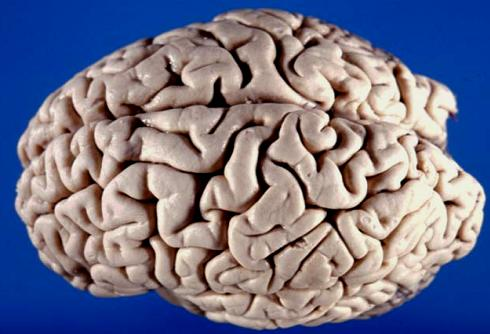
\includegraphics[width=\linewidth]{brain_top.jpg}
    \end{column}
    \begin{column}{0.3\textwidth}
      \onslide<2->{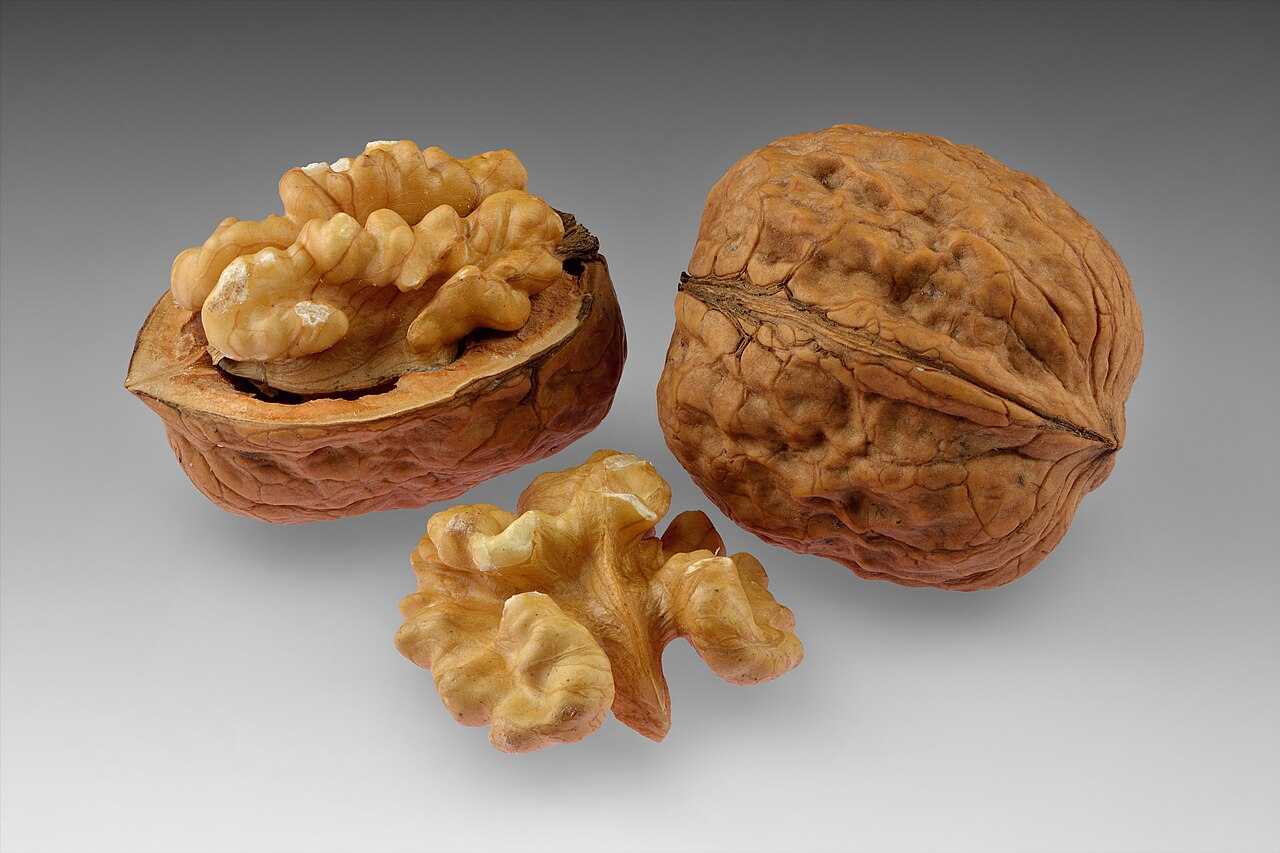
\includegraphics[width=\linewidth]{walnut.jpg}}
    \end{column}
    \begin{column}{0.32\textwidth}
      \onslide<3->{%
      \begin{bookquote}
        Բավական է նայել այս բանին, հասկանալու համար, թե որքան ծիծաղելի է այն. նման է \textbf{մուտանտ ընկույզի}, ծեր բռնցքամարտի ձեռնոցի...
      \end{bookquote}}
    \end{column}
  \end{columns}
  \vspace{5mm}
  \onslide<4->{%
  \begin{card}[colback=butter!45!cream]
    \centering Ապշեցուցիչ է, բայց \textbf{հեռու է կատարյալ լինելուց}։ Եվ այդ թերությունները ազդում են ամեն ինչի վրա, ինչ ասում, անում ու զգում ենք։
  \end{card}}
\end{frame}

% Evolution leaves junk behind: the old hard drive
\begin{frame}{Հին համակարգիչ՝ լիքը աղբով}
  \begin{columns}[c]
    \begin{column}{0.5\textwidth}
      \begin{itemize}
        \item Ուղեղը միլիոնավոր տարիներ է էվոլյուցիա անցել
        \item Նոր հնարավորությունները ավելացել են \textbf{հների վրայից}, հինը չի ջնջվել
        \item Արդյունքը՝ սովորությունների, հնացած պրոցեսների ու անարդյունավետ համակարգերի խճճված կծիկ
      \end{itemize}
      \vspace{2mm}
      \begin{bookquote}
        Կոշտ սկավառակ, լիքը հին ծրագրերով, որոնց pop-up-ները խանգարում են ամենապարզ գործին։
      \end{bookquote}
    \end{column}
    \begin{column}{0.44\textwidth}
      \begin{tikzpicture}[win/.style={draw=plum, line width=0.8pt, fill=cardwhite, rounded corners=1.5mm,
          minimum width=4.6cm, minimum height=1.3cm, text width=4.2cm, align=left, font=\small, inner sep=2mm}]
        \foreach \i/\t in {0/Վա՜խ։ Կարող է վագր լինի, 1/Թույն է։ Փսխե՛լ, 2/Ինչի՞ համար էիր եկել, 3/Աղանդերի տեղ միշտ կա}{
          \begin{scope}[shift={(\i*0.42,-\i*1.0)}]
            \fill[plum, rounded corners=1.5mm] (0.12,-0.12) rectangle ++(4.6,1.3);
            \node[win, anchor=south west] at (0,0) {};
            \fill[brainpink, rounded corners=1.5mm] (0,0.9) rectangle ++(4.6,0.4);
            \draw[plum, line width=0.8pt] (0,0.9) -- ++(4.6,0);
            \node[anchor=west, font=\blackfont\scriptsize] at (0.1,1.1) {\emoji[0.9em]{warning} ուղեղ.exe};
            \node[anchor=west, font=\small, text=plum] at (0.15,0.43) {\t};
          \end{scope}}
      \end{tikzpicture}
    \end{column}
  \end{columns}
\end{frame}

% Myth or fact: stress can help
\begin{frame}{Առասպել, թե՞ փաստ}
  \mythorfact{Սթրեսը կարող է բարելավել արդյունքը}{ՓԱՍՏ}{mintdark}{%
    \begin{card}[colback=mint!35!cardwhite]
      Դա նյարդաբանական պրոցես է, ոչ թե «խոսք»։ Վերջնաժամկետները (դեդլայնները) սթրես են ստեղծում, ու աշխատանքը հաճախ \textbf{լավանում է}։\par\smallskip
      {\small Բըրնեթ՝ «Եթե գրքի վերջին գլուխները հանկարծ լավանան, հիմա գիտեք՝ ինչու»։}
    \end{card}}
\end{frame}

% Why bother: the two goals of the book
\begin{frame}{Ինչու՞ իմանալ ուղեղի «բագերի» մասին}
  \begin{columns}[T]
    \begin{column}{0.47\textwidth}
      \begin{card}[colback=mint!35!cardwhite]
        \bigemoji[1cm]{bulb}\par\smallskip
        {\blackfont Հասկանալ}\par
        ինչու են մարդիկ (ու դու ինքդ) հաճախ անում ու ասում տարօրինակ բաներ
      \end{card}
    \end{column}
    \begin{column}{0.47\textwidth}
      \begin{card}[colback=lavender!40!cardwhite]
        \bigemoji[1cm]{monocle}\par\smallskip
        {\blackfont Կասկածել}\par
        «նեյրո»-ով սկսվող հրաշք պնդումներին, որոնք գնալով շատանում են
      \end{card}
    \end{column}
  \end{columns}
  \vspace{5mm}
  \centering
  \onslide<2->{\mascot[1.6cm]{happy}\quad\raisebox{0.7cm}{\large Ուղեղի թերությունները ոչ թե թաքցնել, այլ \textbf{ուսումնասիրել} արժե}}
\end{frame}
